\section{Bayesian Statistics}
In classical statistics, model parameters such as $\mu$ and $\sigma$ are treated as constants; \textbf{Bayesian statistics}, on the other hand assume that \textbf{model parameters are random variables}. \newl \textbf{Bayes' Theorem} lies at the foundation of such statistics: 
\begin{equation}\label{eq:Bayes}
    P(H\mid D)=\frac{P(D\mid H)\times P(H)}{P(D)},
\end{equation}
where $H$ represents the hypothesis and $D$ denotes the observed data, which is sometimes written in shorthand as  $P(H\mid D) \propto P(D\mid H)\times P(H)$; in other words, our \textbf{degree of belief in a hypothesis should be updated by the evidence provided by the data}.\footnote{Nobody disputes the validity of Bayes' Theorem, and it has proven to be a useful component in various models and algorithms, such as email spam filters, and the following example, but the \textbf{use} of Bayesian statistics is controversial in many quarters.} More details are provided in \cite{DSRS_BDA}.\newl 
Suppose we are interested in diagnosing whether a tumour is begin or malignant, based on several measurements obtained from video imaging. Bayes' Theorem (\ref{eq:Bayes}) can be recast in a tumour data mould:
 \begin{figure*}[!t]
    \centering
      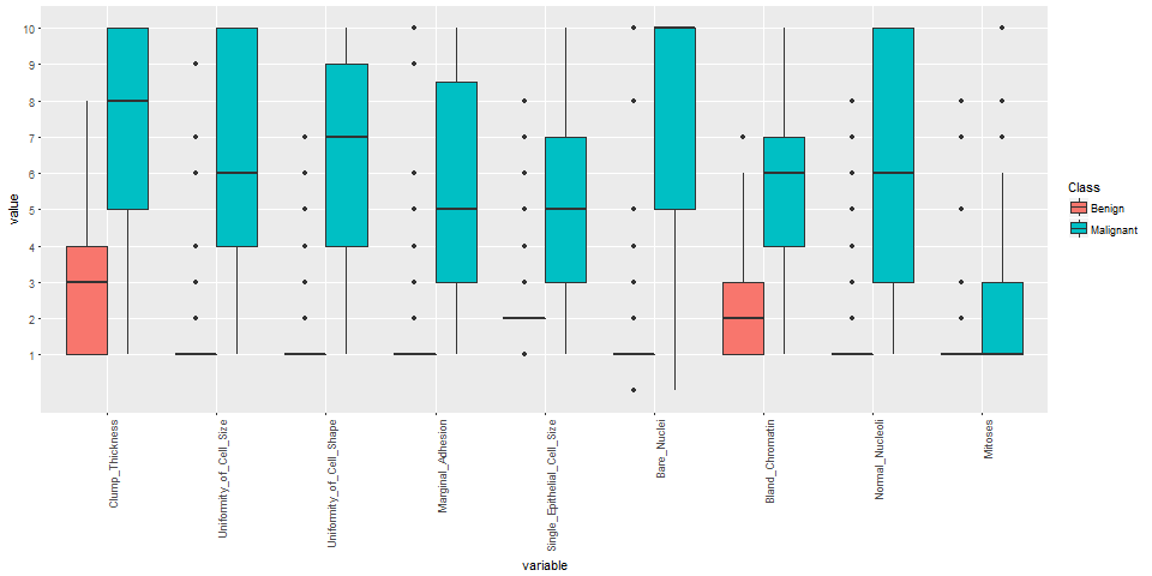
\includegraphics[width=\textwidth]{Images/testA10.png}
      \caption[\small Visualisation of tumour measurements]{\small Boxplot visualisation of measurements for benign and malignant tumours.}
      \label{fig:testA10}
    \end{figure*}
    
    \begin{table*}[!t]
    \centering
      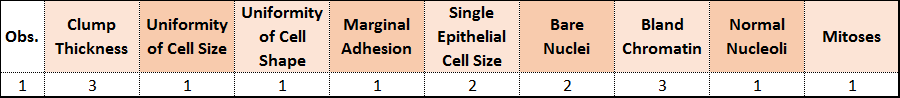
\includegraphics[width=\textwidth]{Images/testA12.png}
      \caption[\small Scores for an undiagnosed tumour]{\small Scores for an undiagnosed tumour.}
      \label{fig:testA12}\hrule
    \end{table*}
\afterpage{\FloatBarrier}
\begin{itemize}[noitemsep]
    \item \textbf{posterior:} $P(H\mid D)=$ based on collected data, how likely is a given tumour to be benign (or malignant)?
    \item \textbf{prior:} $P(H)=$ in what proportion are tumours benign (or malignant) in general? 
    \item \textbf{likelihood:} $P(D\mid H)=$ knowing a tumour is benign (or malignant), how likely is it that these particular measurements would have been observed?
    \item \textbf{evidence:} $P(D)=$ regardless of a tumour being benign or malignant, what is the chance that a tumour has the observed characteristics?
\end{itemize}
To answer the above question (that is, to compute the posterior), we will use a \textbf{na\"{\i}ve Bayes classifier} (NBC; see \cite{DAL_DSML} for more information on  classification methods).

    \subsection{Na\"{\i}ve Bayes Classification for Tumour Diagnoses} The procedure to apply NBC is straightforward. 
\begin{enumerate}
    \item \textbf{Objective function:} a simple way to determine whether a tumour is benign or malignant is to compare \textbf{posterior probabilities} and choose the one with highest probability. That is, we diagnose a tumour as \textbf{malignant} if 
        \begin{equation*}
        \frac{P(\textrm{malignant}\mid D)}{P(\textrm{benign}\mid D)}=\frac{P(D\mid \textrm{malignant})\times P(\textrm{malignant})}{P(D\mid \textrm{benign})\times P(\textrm{benign})}>1,
    \end{equation*}
    and as \textbf{benign} otherwise. 
    
    \item \textbf{Dataset:} the classifier is built on a sample of $N=458$ tumours with nine measurements, each scored on a scale of 1 to 10. The measurements include items such as \textit{clump thickness} and \textit{bare nuclei}; boxplots of these measurements are shown in Figure~\ref{fig:testA10}. We also have undiagnosed cases -- an example of an  \textbf{explanatory signature scores} is given in Table~\ref{fig:testA12}; this is an observation for which a prediction is required.    
   
    \begin{figure*}[!t]
    \centering
      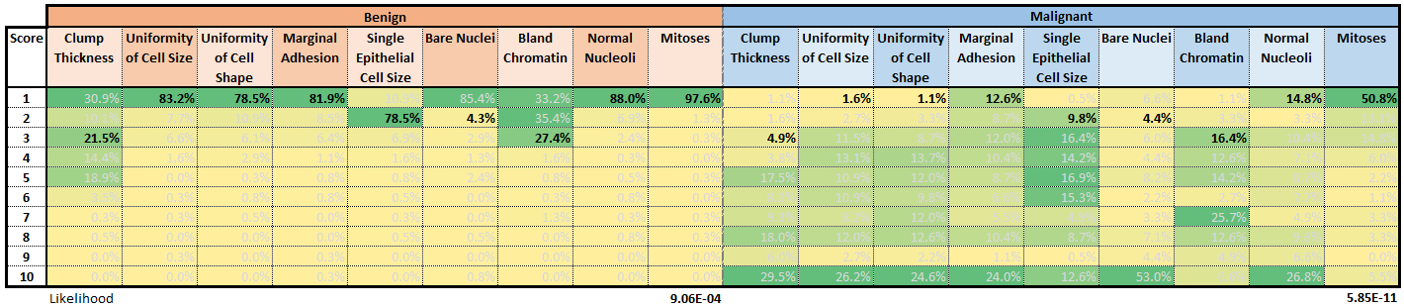
\includegraphics[width=1\linewidth]{Images/testA13.png}
      \caption[\small Multinomial probabilities for benign and malignant tumours]{\small Multinomial probabilities for benign and malignant tumours.}
      \label{fig:testA13}
    \end{figure*}
        \begin{table*}[!t]
        \centering
        \begin{tabular}{c c c c c}
        \hline
        \textbf{Class} & \textbf{Prior} & \textbf{Likelihood} & \textbf{Posterior} & \textbf{Ratio}\\
        \hline
            \textbf{Malignant} & $0.327$ & $5.85\times 10^{-11}$ & $1.92\times 10^{-11}$ & $3.15 \times 10^{-8}$\\
        \textbf{Benign} & $0.673$ & $9.06\times 10^{-4}$ & $6.09\times 10^{-4}$ \\

        \hline
        \end{tabular}
        \caption[\small Computation of posterior probabilities in the undiagnosed case]{\small Computation of posterior probabilities in the undiagnosed case of Table~\ref{fig:testA12}.}
        \label{tab:SA9}\hrule
     \end{table*}  
    \item \textbf{Assumptions:} we assume that the scores of each measurement are independent of one another (hence the \textbf{naive} qualifier); this assumption reduces the likelihood function to
    \begin{align*}
        P(H\mid D)&=P(H\mid x_{1},x_{2},\cdots,x_{9})\\&=P(H\mid x_{1})\times \cdots\times P(H\mid x_{9}).
    \end{align*}
    \item \textbf{Prior distribution:} we can ask subject matter experts to provide a rough estimate for the general ratio of benign to malignant tumours, or use the proportion of benign tumours in the sample as our prior. In situations where we have no knowledge about the distribution of priors, we may simply assume a \textbf{non-informative prior} (in this case, the prevalence rates would be the same for both responses). 
    
    \item \textbf{Computation of likelihoods:} under independence, each measurement is assumed to follow a multinomial distribution (since scores are on $1-10$ scale). Multiplying probabilities from each multinomial distribution (one each for both classes) provides the overall likelihoods for benign and malignant tumours, respectively. The likelihood of the undiagnosed case being a benign tumour is seen to be $9.06\times 10^{-4}$, while the likelihood of being a malignant tumour is $5.85\times 10^{-11}$, based on the multinomial probabilities given in Table~\ref{fig:testA13}
    

    
    
    \item \textbf{Computation of Posterior:} Multiplying the prior probability and likelihood, we get a quqntity that is proportional to the respective posterior probabilities. Looking at Table \ref{tab:SA9}, we conclude that the tumour in the undiagnosed case is \textbf{likely benign} (note that we have no measurement on how much more likely it is to be benign than to be malignant -- the classifier is \textbf{not calibrated}).
    
  
        
\end{enumerate}

